\chapter{Governing Equations}\label{ch:GovEq}
\section{The Euler Equations}
The Euler equations are a system of time dependent non-linear hyperbolic partial differential equations that govern the dynamics of inviscid fluid flow. The five governing equations are the conservation of mass, $x$-momentum, $y$-momentum, $z$-momentum, and energy.
\begin{equation}
	\rho_t  + \left(\rho u\right)_x  + \left(\rho v\right)_y  + \left(\rho w\right)_z = 0
\end{equation}
\begin{equation}
	\left(\rho u\right)_t + \left(\rho u^2 + p\right)_x + \left(\rho u v\right)_y + \left(\rho u w\right)_z = 0
\end{equation}
\begin{equation}
	\left(\rho v\right)_t + \left(\rho u v + p\right)_x + \left(\rho v^2 + p\right)_y + \left(\rho v w\right)_z = 0
\end{equation}
\begin{equation}
	\left(\rho w\right)_t + \left(\rho u w + p\right)_x + \left(\rho v w\right)_y + \left(\rho w^2 + p\right)_z = 0
\end{equation}
\begin{equation}
	E_t + \left[u\left(E + p\right)\right]_x + \left[v\left(E + p\right)\right]_y + \left[w\left(E + p\right)\right]_z = 0
\end{equation}
This system of PDEs can be represented more compactly using the vector definitions for the quantities
\begin{equation}
	\boldsymbol{U} =
	\begin{bmatrix}
		\rho\\
		\rho u\\
		\rho v\\
		\rho w\\
		E
	\end{bmatrix},\,\,
	\boldsymbol{F} =
	\begin{bmatrix}
		\rho u\\
		\rho u^2 + p\\
		\rho u v\\
		\rho u w\\
		u\left(E + p\right)
	\end{bmatrix},\,\,
	\boldsymbol{G} =
	\begin{bmatrix}
		\rho u\\
		\rho u v\\
		\rho v^2 + p\\
		\rho v w\\
		v\left(E + p\right)
	\end{bmatrix},\,\,
	\boldsymbol{H} =
	\begin{bmatrix}
		\rho u\\
		\rho u w\\
		\rho v w\\
		\rho w^2 + p\\
		w\left(E + p\right)
	\end{bmatrix}
\end{equation}
Where $E$ is the total energy per unit volume and is defined as
\begin{equation}
	E = \frac{1}{2} \rho \boldsymbol{V}^2 + pe
\end{equation}
and $\boldsymbol{V}^2$ is
\begin{equation}
	\boldsymbol{V}^2 = u^2 + v^2 + w^2
\end{equation}
and the specific internal energy, $e$, for an ideal gas is
\begin{equation}\label{eqn:idealgasEOS}
	e = \frac{p}{\left(\gamma - 1\right) \rho}
\end{equation}
So that the system of PDEs can take the more compact vector form
\begin{equation}\label{eqn:EulerVector}
	\boldsymbol{U}_t + \boldsymbol{F}\left(\boldsymbol{U}\right)_x + \boldsymbol{G}\left(\boldsymbol{U}\right)_y + \boldsymbol{H}\left(\boldsymbol{U}\right)_z = \boldsymbol{0}
\end{equation}
The integral form of the conservation laws are
\begin{equation}\label{eq:IntegralForm}
	\frac{d}{dt} \int \int \int_{V} \boldsymbol{U} d V + \int \int_A \mathcal{H} \boldsymbol{\cdot} \boldsymbol{n} d A = \boldsymbol{0}
\end{equation}
where $\mathcal{H} = \left(\boldsymbol{F},\boldsymbol{G},\boldsymbol{H}\right)$ is the tensor of fluxes. In the one-dimensional case, the Euler equations take the form
\begin{equation}\label{eqn:EulerVector1d}
	\boldsymbol{U}_t + \boldsymbol{F}\left(\boldsymbol{U}\right)_x = \boldsymbol{0}
\end{equation}
Where the one-dimensional form of $\boldsymbol{U}$ and $\boldsymbol{F}$ are
\begin{equation}
	\boldsymbol{U} =
	\begin{bmatrix}
		\rho\\
		\rho u\\
		E
	\end{bmatrix},\,\,
	\boldsymbol{F} =
	\begin{bmatrix}
		\rho u\\
		\rho u^2 + p\\
		u\left(E + p\right)
	\end{bmatrix}
\end{equation}
The Euler equations can be linearized, so that the equations can be represented in the following form
\begin{equation}\label{eqn:LinEuler}
	\boldsymbol{U}_t + \boldsymbol{A} \boldsymbol{U}_x = \boldsymbol{0}
\end{equation}
by finding a matrix, $\boldsymbol{A}$, where
\begin{equation}\label{eq:LinEquiv}
	\boldsymbol{F} = \boldsymbol{A}\boldsymbol{U}
\end{equation}
The matrix, $\boldsymbol{A}$, is the Jacobian matrix given by
\begin{equation}\label{eqn:JacobDef}
	\boldsymbol{A} = \frac{\partial \boldsymbol{F}}{\partial \boldsymbol{U}}
\end{equation}
To find $\frac{\partial \boldsymbol{F}}{\partial \boldsymbol{U}}$the components of $\boldsymbol{F}$ must be represented by the components of $\boldsymbol{U}$.
\begin{equation}
	\rho = u_1
\end{equation}
\begin{equation}
	\rho u = u_2
\end{equation}
\begin{equation}
	E = u_3
\end{equation}
Then $u$ and $a$ can be represented as
\begin{equation}
	u = \frac{u_2}{u_1}
\end{equation}
\begin{equation}
	a = \sqrt{\left(\frac{u_3}{u_1} - \frac{1}{2} \left(\frac{u_2}{u_1}\right)^2\right)\left(\gamma\left(\gamma - 1\right)\right)}
\end{equation}
so that $\boldsymbol{F}$ becomes
\begin{equation}
	\boldsymbol{F} =
	\begin{bmatrix}
		u_2\\
		\frac{u_2^2}{2 u_1} \left(3 - \gamma\right) + u_3 \left(\gamma - 1\right)\\
		\gamma \frac{u_2}{u_1} u_3 - \frac{u_2^3}{2 u_1^2} \left(\gamma - 1\right)
	\end{bmatrix}
\end{equation}
The Jacobian matrix can be evaluated according to \equationref{eqn:JacobDef}, given in full by
\begin{equation}
	\boldsymbol{A} = 
	\begin{bmatrix}
		\frac{\partial f_1}{\partial u_1} & \frac{\partial f_1}{\partial u_2} & \frac{\partial f_1}{\partial u_3}\\
		\frac{\partial f_2}{\partial u_1} & \frac{\partial f_2}{\partial u_2} & \frac{\partial f_2}{\partial u_3}\\
		\frac{\partial f_3}{\partial u_1} & \frac{\partial f_3}{\partial u_2} & \frac{\partial f_3}{\partial u_3}
	\end{bmatrix}
\end{equation}
Evaluating the derivatives of the components of $\boldsymbol{F}$ with respect to the components of $\boldsymbol{U}$, gives the following Jacobian matrix for the one-dimensional Euler equations
\begin{equation}
	\boldsymbol{A} = 
	\begin{bmatrix}
		0 & 1 & 0\\
		\frac{u^2}{2}\left(\gamma - 3\right)& u(3 - \gamma) & \gamma - 1\\
		\frac{u^3}{2} \left(\gamma - 2\right) - \frac{a^2 u}{\gamma - 1}& \frac{3 - 2 \gamma}{2} u^2 + \frac{a^2}{\gamma - 1}  & \gamma u
	\end{bmatrix}
\end{equation}
where $a$ is the speed of sound and is given by
\begin{equation}
	a = \sqrt{\frac{\gamma p}{\rho}}
\end{equation}
Allowing the system of PDEs to be represented in the form of \equationref{eqn:LinEuler}.
\section{The Riemann Problem}
The Riemann problem for the one dimensional Euler equations, \equationref{eqn:EulerVector1d}, is an Initial Value Problem with the initial conditions of
\begin{equation}\label{eqn:RiemannProblem}
	\boldsymbol{U}\left(x,0\right) = \begin{cases}
		\boldsymbol{U}_L\,\,\,\, \textrm{ if } \,\,x < 0,\\
		\boldsymbol{U}_R\,\,\,\, \textrm{ if } \,\,x > 0,
	\end{cases}
\end{equation}
This is a generalization of the shock-tube problem for the Euler equations, where two stationary gases ($u_L=u_R=0$), are separated by a membrane, that when removed creates a wave system \cite{courant1999supersonic}. In the Riemann problem, however, the particle velocities, $u_L$ and $u_R$, are allowed to be non-zero \cite{toro2013riemann}.
When defining a Riemann problem, it is sometimes more convenient to refer to  the vector of primitive variables, $\boldsymbol{W}$
\begin{equation}
	\boldsymbol{W} = \begin{bmatrix}
		\rho\\ u\\ p
	\end{bmatrix}
\end{equation}\begin{figure}
	\centering
	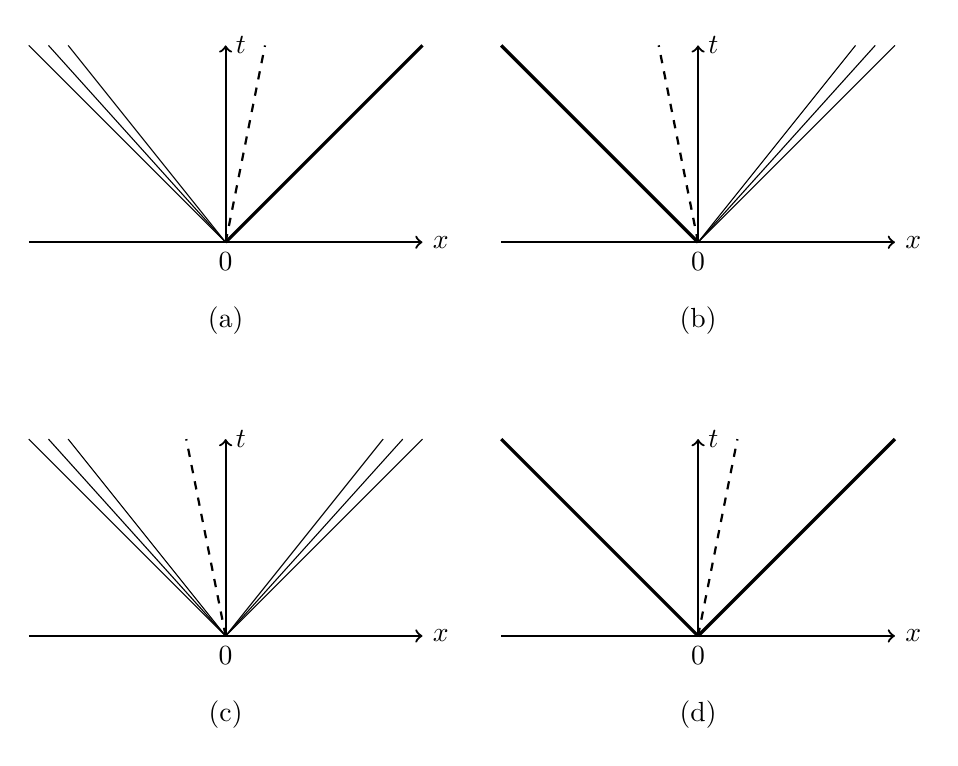
\begin{tikzpicture}[scale=0.25]
		%first
		\draw[thick,->] (-10,0) -- (10,0) node[anchor=west]{$x$};
		\draw[thick,->] (0,0) node[anchor=north]{$0$} -- (0,7) -- (0,9) -- (0,10) node[anchor=west]{$t$};
		\draw[thin,-] (0,0) -- (-10,10);
		\draw[thin,-] (0,0) -- (-9,10);
		\draw[thin,-] (0,0) -- (-8,10);
		\draw[thick,dashed] (0,0) -- (2,10);
		\draw[very thick,-] (0,0) -- (10,10);
		\node at (0,-4) {(a)};
		%second
		\draw[thick,->] (14,0) -- (34,0) node[anchor=west]{$x$};
		\draw[thick,->] (24,0) node[anchor=north]{$0$} -- (24,7) -- (24,9) -- (24,10) node[anchor=west]{$t$};
		\draw[thin,-] (24,0) -- (34,10);
		\draw[thin,-] (24,0) -- (33,10);
		\draw[thin,-] (24,0) -- (32,10);
		\draw[thick,dashed] (24,0) -- (22,10);
		\draw[very thick,-] (24,0) -- (14,10);
		\node at (24,-4) {(b)};
		%third
		\draw[thick,->] (-10,-20) -- (10,-20) node[anchor=west]{$x$};
		\draw[thick,->] (0,-20) node[anchor=north]{$0$} -- (0,-13) -- (0,-11) -- (0,-10) node[anchor=west]{$t$};
		\draw[thin,-] (0,-20) -- (-10,-10);
		\draw[thin,-] (0,-20) -- (-9,-10);
		\draw[thin,-] (0,-20) -- (-8,-10);
		\draw[thick,dashed] (0,-20) -- (-2,-10);
		\draw[thin,-] (0,-20) -- (10,-10);
		\draw[thin,-] (0,-20) -- (9,-10);
		\draw[thin,-] (0,-20) -- (8,-10);
		\node at (0,-24) {(c)};
		%fourth
		\draw[thick,->] (14,-20) -- (34,-20) node[anchor=west]{$x$};
		\draw[thick,->] (24,-20) node[anchor=north]{$0$} -- (24,-13) -- (24,-11) -- (24,-10) node[anchor=west]{$t$};
		\draw[very thick,-] (24,-20) -- (34,-10);
		\draw[thick,dashed] (24,-20) -- (26,-10);
		\draw[very thick,-] (24,-20) -- (14,-10);
		\node at (24,-24) {(d)};
	\end{tikzpicture}
	\caption[Configuration of the wave system: (a) Left rarefaction, contact, right shock. (b) Left shock, contact, right rarefaction. (c) Left rarefaction, contact, right rarefaction. (d) Left shock, contact, right shock.]{Configuration of the wave system: (a) Left rarefaction, contact, right shock. (b) Left shock, contact, right rarefaction. (c) Left rarefaction, contact, right rarefaction. (d) Left shock, contact, right shock.}
	\label{fig:WaveConfig}
\end{figure}
Where, as in the case of \equationref{eqn:RiemannProblem}, the left and right states, $\boldsymbol{W}_L$ and $\boldsymbol{W}_R$, are separated by a discontinuity at $x = 0$. For an ideal gas that obeys the caloric equation of state in \equationref{eqn:idealgasEOS}, the wave system created by the removal of the membrane has four possible configurations of waves seen in \figureref{fig:WaveConfig}. The wave system can consist of left and right rarefaction waves, left and right shock waves or a combination of the two \cite{toro2013riemann}. As can be viewed in \figureref{fig:SolutionStructure}, the left and right waves are separated by a contact discontinuity. The unknown regions between the left and right states are referred to as the star region, which contains the left and right star states, $\boldsymbol{W}_{*L}$ and $\boldsymbol{W}_{*L}$. An iterative solver for the Riemann problem is presented in \sectionref{sect:AdaptiveRiemannSolver}.
\begin{figure}
	\centering
	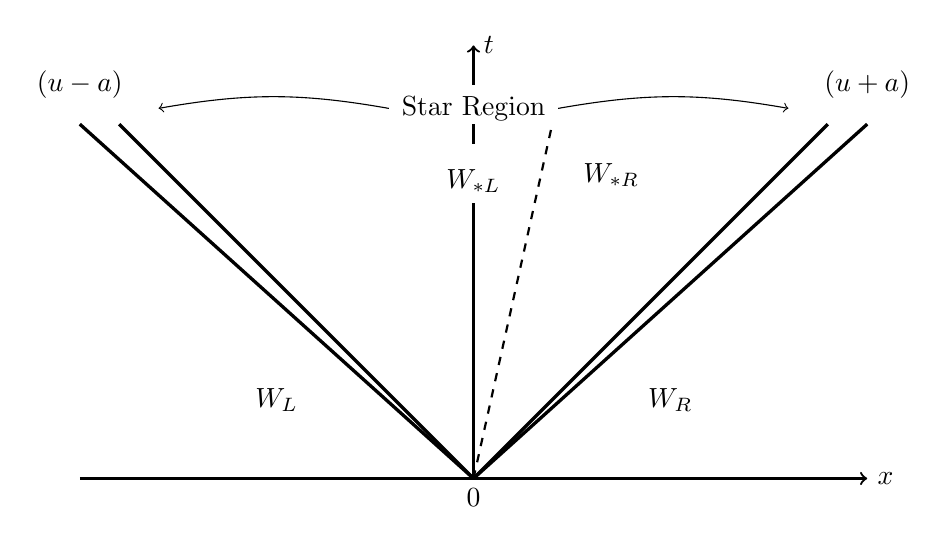
\begin{tikzpicture}[scale=0.5]
		\draw[thick,->] (-10,0) -- (10,0) node[anchor=west]{$x$};
		\draw[thick,-] (0,0)node[anchor=north]{$0$} -- (0,7)node[anchor=south]{$\boldsymbol{W}_{*L}$};
		\draw[thick,-] (0,8.5) -- (0,9);
		\draw[thick,->] (0,10) -- (0,11) node[anchor=west]{$t$};
		\node at (3.5,7.7){$\boldsymbol{W}_{*R}$};
		\draw[very thick,-] (0,0) -- (10,9);
		\draw[very thick,-] (0,0) -- (9,9);
		\draw[thick,dashed] (0,0) -- (2,9);
		\draw[very thick,-] (0,0) -- (-9,9);
		\draw[very thick,-] (0,0) -- (-10,9);
		\node at (-10,10){$\left(u-a\right)$};
		\node at (10,10){$\left(u+a\right)$};
		\node at (-5,2){$\boldsymbol{W}_{L}$};
		\node at (5,2){$\boldsymbol{W}_{R}$};
		\draw[thin,->] (-2.15,9.4) to [out=170,in=10] (-8,9.4);
		\draw[thin,->] (2.15,9.4) to [out=10,in=170] (8,9.4);
		\node at (0,9.4){Star Region};
	\end{tikzpicture}
	\caption[Solution structure of the Riemann problem on the $x$-$t$ plane for the time-dependent Euler equations.]{Solution structure of the Riemann problem on the $x$-$t$ plane for the time-dependent Euler equations.}
	\label{fig:SolutionStructure}
\end{figure}
%\begin{figure}
%\begin{tikzpicture}[scale=0.2]
%\end{tikzpicture}
%\caption[Wave Configuration 2: Left shock wave, centered contact discontinuity, and a right rarefaction wave.]{Wave Configuration 2: Left shock wave, centered contact discontinuity, and a right rarefaction wave.}
%\label{fig:RightTransonicRarefaction}
%\end{figure}
%\begin{figure}
%\begin{tikzpicture}[scale=0.2]
%	\draw[thick,->] (-10,0) -- (10,0) node[anchor=west]{$x$};
%	\draw[thick,->] (0,0) node[anchor=north]{$0$} -- (0,7) -- (0,9) -- (0,10) node[anchor=west]{$t$};
%	\draw[thin,-] (0,0) -- (-10,10);
%	\draw[thin,-] (0,0) -- (-9,10);
%	\draw[thin,-] (0,0) -- (-8,10);
%	\draw[thick,dashed] (0,0) -- (2,10);
%	\draw[thin,-] (0,0) -- (10,10);
%	\draw[thin,-] (0,0) -- (9,10);
%	\draw[thin,-] (0,0) -- (8,10);
%\end{tikzpicture}
%\caption[Wave Configuration 3: Left rarefaction wave, centered contact discontinuity, and a right rarefaction wave.]{Wave Configuration 3: Left rarefaction wave, centered contact discontinuity, and a right rarefaction wave.}
%\label{fig:TwoRarefaction}
%\end{figure}
%\begin{figure}
%\begin{tikzpicture}[scale=0.2]
%	\draw[thick,->] (-10,0) -- (10,0) node[anchor=west]{$x$};
%	\draw[thick,->] (0,0) node[anchor=north]{$0$} -- (0,7) -- (0,9) -- (0,10) node[anchor=west]{$t$};
%	\draw[very thick,-] (0,0) -- (10,10);
%	\draw[thick,dashed] (0,0) -- (-2,10);
%	\draw[very thick,-] (0,0) -- (-10,10);
%\end{tikzpicture}
%\caption[Wave Configuration 4: Left shock wave, centered contact discontinuity, and a right shock wave.]{Wave Configuration 4: Left shock wave, centered contact discontinuity, and a right shock wave.}
%\label{fig:TwoShock}
%\end{figure}
\section{The Approximate Riemann Problem}
For a linear hyperbolic system with constant coefficients, the difference in the conservative variables can be written as
\begin{equation}
	\Delta \boldsymbol{U} = \boldsymbol{U}_R - \boldsymbol{U}_L
\end{equation}
Which when projected onto the right eigenvectors of the Jacobian Matrix, $\tilde{\boldsymbol{A}}$, becomes
\begin{equation}\label{eqn:datadifference}
	\Delta \boldsymbol{U} = \boldsymbol{U}_R - \boldsymbol{U}_L = \sum_{i=1}^m \tilde{\alpha}_i \tilde{\boldsymbol{K}}^{\left(i\right)}
\end{equation}
Where $\tilde{\alpha}_i$ are the associated wave strengths. The values of $\boldsymbol{U}_{i+\frac{1}{2}}$ are evaluated using the equations
\begin{equation}\label{eqn:Usum1}
	\boldsymbol{U}_{i+\frac{1}{2}}\left(0\right) = \boldsymbol{U}_L + \sum_{\tilde{\lambda}_i \le 0} \tilde{\alpha}_i \tilde{\boldsymbol{K}}^{\left(i\right)}
\end{equation}
or from
\begin{equation}\label{eqn:Usum2}
	\boldsymbol{U}_{i+\frac{1}{2}}\left(0\right) = \boldsymbol{U}_R - \sum_{\tilde{\lambda}_i \ge 0} \tilde{\alpha}_i \tilde{\boldsymbol{K}}^{\left(i\right)}
\end{equation}
Replacing the original system of equations, \equationref{eqn:EulerVector1d}, with a modified linear system with constant coefficients, \equationref{eqn:LinEuler}, we have a modified system
\begin{equation}
	\tilde{\boldsymbol{U}}_t + \tilde{\boldsymbol{F}}\left(\tilde{\boldsymbol{U}}\right)_x = \boldsymbol{0}
\end{equation}
with a flux function
\begin{equation}\label{eqn:FluxDef}
	\tilde{\boldsymbol{F}}\left(\tilde{\boldsymbol{U}}\right) = \tilde{\boldsymbol{A}}\tilde{\boldsymbol{U}}
\end{equation}
The corresponding numerical flux, $\boldsymbol{F}$, is found from the following relations
\begin{equation}\label{eqn:flux1}
	\boldsymbol{F}_{0L} = \boldsymbol{F}_L - S_L \boldsymbol{U}_L - \frac{1}{T} \int_{TS_L}^{0} \boldsymbol{U}\left(x,T\right)\,dx
\end{equation}
\begin{equation}\label{eqn:flux2}
	\boldsymbol{F}_{0R} = \boldsymbol{F}_R - S_R \boldsymbol{U}_R + \frac{1}{T} \int_{0}^{TS_R} \boldsymbol{U}\left(x,T\right)\,dx
\end{equation}
Where $S_R$ and $S_L$ are the largest and smallest wave speeds in the exact solution of the Riemann problem that has the right and left states $\boldsymbol{U}_R$ and $\boldsymbol{U}_L$ and $T$ is some positive time. If $\boldsymbol{U}_{i+\frac{1}{2}} \left(x,t\right)$ is a solution of the Riemann problem for the system given in \equationref{eqn:EulerVector1d}, the integral relations in \equationref{eqn:flux1} and \equationref{eqn:flux2} become
\begin{equation}\label{eqn:flux12}
	\int_{TS_L}^{0} \tilde{\boldsymbol{U}}\left(x,T\right)\,dx = T\left[\tilde{\boldsymbol{F}}\left(\boldsymbol{U}_L\right) - \tilde{\boldsymbol{F}}\left(\tilde{\boldsymbol{U}}_{i+\frac{1}{2}}\right)\right] - T S_L \boldsymbol{U}_L
\end{equation}
\begin{equation}\label{eqn:flux22}
	\int_{0}^{TS_R} \tilde{\boldsymbol{U}}\left(x,T\right)\,dx = T\left[\tilde{\boldsymbol{F}}\left(\tilde{\boldsymbol{U}}_{i+\frac{1}{2}}\right) - \tilde{\boldsymbol{F}}\left(\boldsymbol{U}_R\right)\right] + T S_R \boldsymbol{U}_R
\end{equation}
Substituting \equationref{eqn:flux12} and \equationref{eqn:flux22} into \equationref{eqn:flux1} and \equationref{eqn:flux2} gives the following
\begin{equation}\label{eqn:flux13}
	\boldsymbol{F}_{0L} = \tilde{\boldsymbol{F}}\left(\tilde{\boldsymbol{U}}_{i+\frac{1}{2}}\left(0\right)\right) + \boldsymbol{F}\left(\boldsymbol{U}_L\right) - \tilde{\boldsymbol{F}}\left(\boldsymbol{U}_L\right)
\end{equation}
\begin{equation}\label{eqn:flux23}
	\boldsymbol{F}_{0R} = \tilde{\boldsymbol{F}}\left(\tilde{\boldsymbol{U}}_{i+\frac{1}{2}}\left(0\right)\right) + \boldsymbol{F}\left(\boldsymbol{U}_R\right) - \tilde{\boldsymbol{F}}\left(\boldsymbol{U}_R\right)
\end{equation}
Using $\tilde{\boldsymbol{U}}_{i+\frac{1}{2}}\left(0\right)$ from \equationref{eqn:Usum1} or from \equationref{eqn:Usum2} and using \equationref{eqn:FluxDef} the numerical flux is given by
\begin{equation}\label{eqn:Fsum1}
	\boldsymbol{F}_{i+\frac{1}{2}} = \boldsymbol{F}_L + \sum_{\tilde{\lambda}_i \le 0} \tilde{\alpha}_i  \tilde{\lambda}_i  \tilde{\boldsymbol{K}}^{\left(i\right)}
\end{equation}
or from
\begin{equation}\label{eqn:Fsum2}
	\boldsymbol{F}_{i+\frac{1}{2}} = \boldsymbol{F}_R - \sum_{\tilde{\lambda}_i \ge 0} \tilde{\alpha}_i  \tilde{\lambda}_i  \tilde{\boldsymbol{K}}^{\left(i\right)}
\end{equation}
The simple arithmetic average of the numerical flux definitions of \equationref{eqn:Fsum1} and \equationref{eqn:Fsum2} used in the computation is
\begin{equation}\label{eqn:NumericalFluxAverage}
	\boldsymbol{F}_{i+\frac{1}{2}} = \frac{1}{2} \left( \boldsymbol{F}_L + \boldsymbol{F}_R \right)- \frac{1}{2}\sum_{i = 1}^{m} \tilde{\alpha}_i  |\tilde{\lambda}_i |  \tilde{\boldsymbol{K}}^{\left(i\right)}
\end{equation}